\documentclass[tikz,border=3pt]{standalone}
\usepackage[utf8]{inputenc}
\usepackage[T1]{fontenc}
\usepackage{lmodern}
\renewcommand{\familydefault}{\sfdefault}
\usepackage{sansmath}\sansmath
\usepackage{chemfig}
\usepackage{pgfplots}\pgfplotsset{compat=1.18,/pgf/number format/use comma,/pgf/number format/1000 sep={.}}
\usetikzlibrary{arrows.meta,calc,positioning,decorations.pathmorphing,patterns}
% paleta del sitio
\definecolor{nar}{HTML}{E8680C}\definecolor{narc}{HTML}{FFB35C}\definecolor{hielo}{HTML}{FFF3E8}
\definecolor{tinta}{HTML}{1D1D1F}\definecolor{gris}{HTML}{6E6E73}\definecolor{lila}{HTML}{7C5CF0}
\definecolor{azul}{HTML}{2F6FD6}\definecolor{menta}{HTML}{17A673}\definecolor{coral}{HTML}{E8342A}
\begin{document}
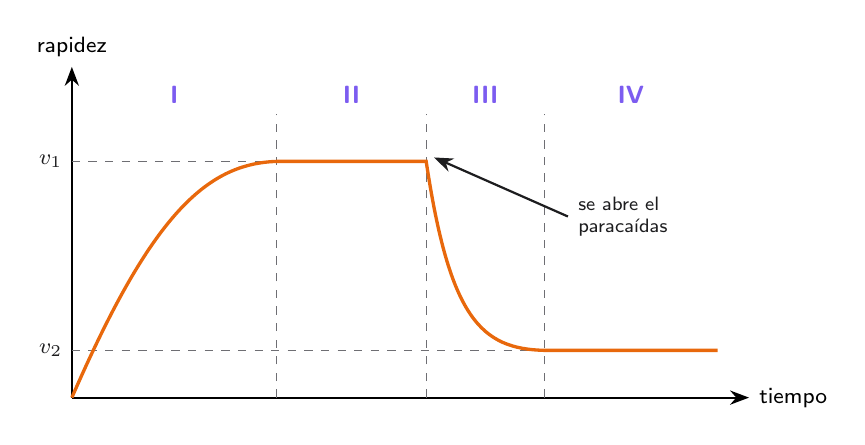
\begin{tikzpicture}[font=\footnotesize,>={Stealth[length=2.4mm]}]
\draw[->,thick] (0,0) -- (8.6,0) node[right] {tiempo};
\draw[->,thick] (0,0) -- (0,4.2) node[above] {rapidez};
\draw[dashed,gris] (0,3) node[left,text=tinta] {$v_1$} -- (2.6,3);
\draw[dashed,gris] (0,0.6) node[left,text=tinta] {$v_2$} -- (6.0,0.6);
\draw[dashed,gris] (2.6,0) -- (2.6,3.6) (4.5,0) -- (4.5,3.6) (6.0,0) -- (6.0,3.6);
\draw[very thick,nar] (0,0) .. controls (1.0,2.3) and (1.7,2.97) .. (2.6,3) -- (4.5,3)
  .. controls (4.8,1.0) and (5.2,0.62) .. (6.0,0.6) -- (8.2,0.6);
\foreach \x/\l in {1.3/I,3.55/II,5.25/III,7.1/IV} \node[font=\small\bfseries,lila] at (\x,3.85) {\l};
\draw[<-,thick,tinta] (4.6,3.05) -- (6.3,2.3) node[right,align=left,font=\scriptsize] {se abre el\\paracaídas};
\end{tikzpicture}
\end{document}
